\documentclass[11pt]{article}
\usepackage[margin=1in]{geometry}
\usepackage{graphicx,booktabs,amsmath,amssymb,xcolor,enumitem,caption}
\usepackage[colorlinks=true,linkcolor=blue,urlcolor=blue]{hyperref}
\captionsetup{font=small}
\setlength{\parskip}{0.4em}\setlength{\parindent}{0pt}
\newcommand{\J}{\textit{J}}

\title{\vspace{-1.5em}Can a training intervention make a small LM show\\\emph{increasing} returns to experience?\\[0.3em]
\large A sandbox discovery and its test on CHILDES}
\author{Standard Model 2 --- exploratory side-arc}
\date{2026-06-20}

\begin{document}
\maketitle
\vspace{-1.5em}

\section{The question}
Children show \emph{increasing} returns to linguistic experience: harder words are acquired
\emph{faster} later in development (the per-child scaling exponent $\kappa_i \approx 10$ on cumulative
input). Language models, scaled over data, show the opposite --- \emph{diminishing} returns (our
CHILDES developmental ladder gives an effective $\kappa$ falling $\sim$1.3$\to$0.5 over budget). Read
as a \emph{returns-to-experience} exponent, $\kappa<1$ is diminishing (the LM default), $\kappa=1$ a
unit accumulator, and $\kappa>1$ the kid-like ``learning-to-learn'' signature.

\textbf{This side-arc asks a hypothesis-generation question:} is there \emph{any} training intervention
that flips a small from-scratch LM from diminishing toward kid-like increasing returns --- and if so,
is it a genuine learning-to-learn effect or an optimization artifact? We answer in two phases: a fast
sandbox sweep that \emph{finds} a lever, and a controlled CHILDES experiment that \emph{stress-tests}
what it actually does.

\medskip
\textbf{Metric.} For a run we probe per-word mean surprisal at $\sim$log-spaced steps and define
\[
\J \;=\; r_{\text{late}} - r_{\text{early}}
\;=\;\big(\text{slope of } -\text{surprisal on } \log_{10}\text{experience, late half}\big)-\big(\text{same, early half}\big).
\]
$\J<0$ = diminishing returns; $\J\!\approx\!0$ = unit accumulator; $\J>0$ = \textbf{increasing returns}
(the acceleration signature). \textbf{Artifact controls:} $\J>0$ counts only if early learning stayed
healthy ($r_{\text{early}}\!\gtrsim\!0.4$) \emph{and} final competence stayed near baseline --- otherwise a
model that simply learns slowly then ``catches up'' fakes $\J>0$ mechanically.

\section{Phase 1 --- Sandbox sweep (Karpathy \texttt{autoresearch}, ClimbMix GPT-2)}
We repurposed a 5-minute single-GPU GPT-2 training loop (nanochat-style, $\sim$50M params, ClimbMix
web text) to optimize for \emph{acceleration} rather than loss, and swept \textbf{79 variants} across 12
intervention families (repetition, grokfast, weight decay, learning-rate magnitude/schedule, batch
size, depth, init scale, optimizer, attention window, and combinations), scoring \J{} with the
artifact controls above.

\textbf{Result: one robust lever --- a flat, low learning rate.} It is the only family that produced
$\J>0$ while passing both artifact controls, as a clean monotonic dose--response (Fig.~\ref{fig:sandbox}).
The mechanism is a \emph{conjunction}: increasing returns require a \textbf{flat (non-decaying) schedule}
\emph{and} a \textbf{low global LR magnitude} --- neither alone suffices (a decay schedule kills it at any
magnitude; a flat schedule at full magnitude is also insufficient; verified with a flat-vs-decay
$\times$ magnitude $2\times2$). Everything else was null or antagonistic: repetition strongly diminishes
(overfitting); grokfast's $\J>0$ is a slow-start artifact (early learning collapses); schedule
\emph{shape}, depth, batch, and small-init alone do nothing.

\begin{figure}[h]\centering
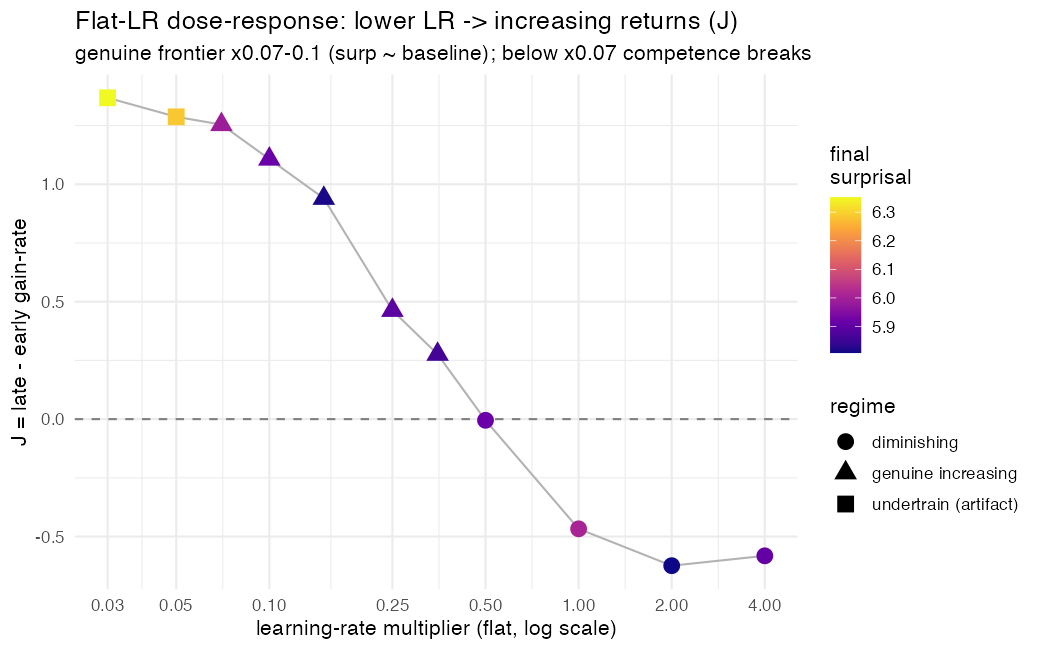
\includegraphics[width=0.78\textwidth]{fig_sandbox_J_vs_LR.png}
\caption{\textbf{Sandbox dose--response.} Lower flat LR $\to$ higher \J{} at maintained competence
(green = passes artifact controls). Below $\sim$0.07$\times$, \J{} keeps rising but competence breaks
(undertraining; orange). On this \emph{web-text} run, the flat-low arms matched baseline on easy
high-frequency words but cost $\sim$0.04--0.09 bits/token of overall validation loss --- they trade
endpoint optimization for a de-front-loaded trajectory.}
\label{fig:sandbox}
\end{figure}

\textbf{The honest caveat from Phase 1.} The flat low LR \emph{mechanically} sustains late-training gains
and de-front-loads the loss curve on the log-experience axis. By our \J{} metric it is the genuine
increasing-returns signature, but whether it is the \emph{same mechanism} as children's increasing
returns was left open --- and it came with a validation-loss cost on web text. Phase 2 was designed to
decide this on real child-directed data, and to add a structural-competence readout (grammar) the
sandbox lacked.

\section{Phase 2 --- Test on CHILDES (GPT-2 small, 24M-word corpus)}
We trained GPT-2 small from scratch on the full $\sim$24M-word CHILDES corpus (the Feng et al.\ setup,
multi-epoch on child-directed speech) and compared a \textbf{standard decayed schedule} (linear decay
from $10^{-4}$) against a \textbf{flat constant schedule} at three magnitudes ($10^{-4},\,3\!\times\!10^{-5},\,10^{-5}$),
$\times$ 2 seeds, at two budgets: \textbf{1$\times$} (20 epochs) and \textbf{4$\times$} (60 epochs; the
``never-finished'' test). Along a shared log-spaced step axis we logged: validation \texttt{bits/token};
\textbf{CDI-word surprisal} $\to$ \J{} (lexical-acquisition axis); \textbf{Zorro} (grammar, \emph{primary} ---
its minimal pairs use a CHILDES-controlled vocabulary, so it isolates syntax from lexical coverage); and
\textbf{BLiMP} (grammar, \emph{secondary/comparability} only --- vocabulary-mismatched to CHILDES, so its
level is depressed and noisy). New tooling: a BLiMP/Zorro minimal-pair scorer and a grammar-trajectory
callback, validated end-to-end.

\begin{table}[h]\centering\small
\caption{Endpoint values (mean over 2 seeds). Lower val\_bpb = better; Zorro/BLiMP higher = better.}
\begin{tabular}{llcccc}
\toprule
budget & schedule (LR) & val\_bpb & Zorro & BLiMP & \J{} \\
\midrule
1$\times$ & decay $10^{-4}$ (standard) & 2.064 & 0.694 & 0.576 & $+0.42$ \\
1$\times$ & flat $10^{-4}$            & 2.225 & 0.674 & 0.576 & $+0.32$ \\
1$\times$ & flat $3\!\times\!10^{-5}$ & 2.030 & 0.701 & 0.577 & $+1.02$ \\
1$\times$ & \textbf{flat $10^{-5}$}   & \textbf{2.017} & 0.690 & 0.589 & $\mathbf{+1.60}$ \\
\midrule
4$\times$ & decay $10^{-4}$ (standard) & \textcolor{red}{2.673} & 0.689 & 0.576 & \textcolor{red}{$-0.60$} \\
4$\times$ & flat $10^{-5}$            & 2.106 & 0.689 & 0.580 & $+1.29$ \\
\bottomrule
\end{tabular}
\label{tab:end}
\end{table}

\section{Results --- four findings}
\textbf{(1) The flat-low-LR increasing-returns signature replicates on CHILDES.}
\J{} rises monotonically as the flat LR drops: flat $10^{-5}$ ($\J\!\approx\!1.60$) $>$ flat $3\!\times\!10^{-5}$
($1.02$) $>$ flat $10^{-4}\!\approx\!$ decay ($\sim$0.3--0.4) (Fig.~\ref{fig:Jdose}). The sandbox dose--response
holds on real data and a real model.

\textbf{(2) On CHILDES, flat-low LR also \emph{wins} validation loss --- flipping the web-text cost.}
flat $10^{-5}$ reaches val\_bpb 2.017 vs.\ the standard schedule's 2.064 (Fig.~\ref{fig:valbpb}); flat
\emph{full}-magnitude is worst (2.225, overfits hardest). This is exactly the regime difference predicted:
CHILDES is small-data \emph{multi-epoch}, where a gentle low LR \textbf{overfits less}, so the sandbox's
endpoint-loss \emph{cost} becomes a \emph{benefit}.

\textbf{(3) The 4$\times$ test is decisive: the standard schedule catastrophically overfits; flat-low is robust.}
With more epochs, standard decay's val\_bpb \emph{worsens} $2.06\!\to\!2.67$ and its \J{} flips
$+0.42\!\to\!-0.60$ (it memorizes, then validation rises). Flat $10^{-5}$ barely moves
($2.02\!\to\!2.11$, $\J$ stays $+1.3$) (Fig.~\ref{fig:overfit}). Flat-low does not ``catch up'' --- it was
already ahead --- but it is the only schedule that survives extended training.

\textbf{(4) Grammar is \emph{decoupled} from all of this.} Zorro plateaus at $\sim$0.68--0.70 for
\emph{every} arm, schedule, and budget (Fig.~\ref{fig:zorro}); BLiMP likewise sits at its CHILDES ceiling
($\sim$0.58). The schedule dramatically reshapes the loss trajectory and the lexical returns (\J{}), but
\textbf{grammatical competence is insensitive to it} --- it reaches its plateau early and stays.

\begin{figure}[h]\centering
\begin{minipage}{0.49\textwidth}\centering
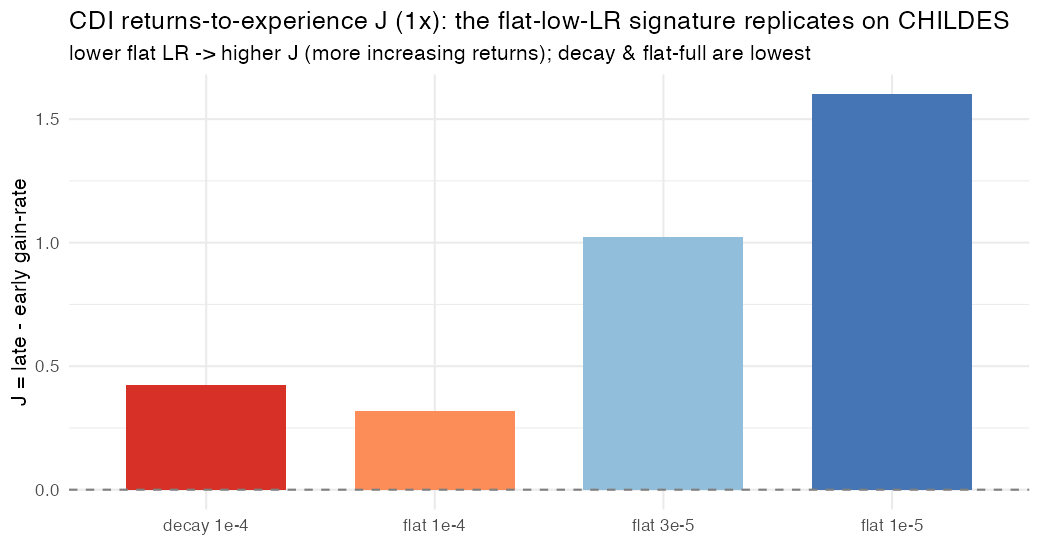
\includegraphics[width=\textwidth]{fig_J_dose.png}\\[-0.2em]
\caption{(1) \J{} dose--response replicates.}\label{fig:Jdose}
\end{minipage}\hfill
\begin{minipage}{0.49\textwidth}\centering
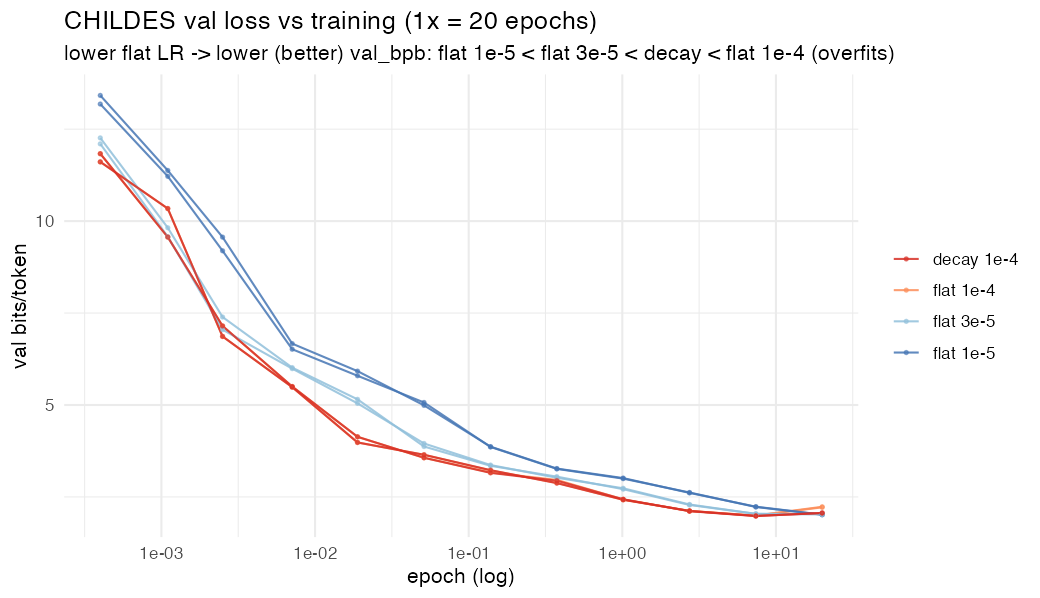
\includegraphics[width=\textwidth]{fig_valbpb_1x.png}\\[-0.2em]
\caption{(2) flat-low wins val loss (anti-overfit).}\label{fig:valbpb}
\end{minipage}
\end{figure}
\begin{figure}[h]\centering
\begin{minipage}{0.49\textwidth}\centering
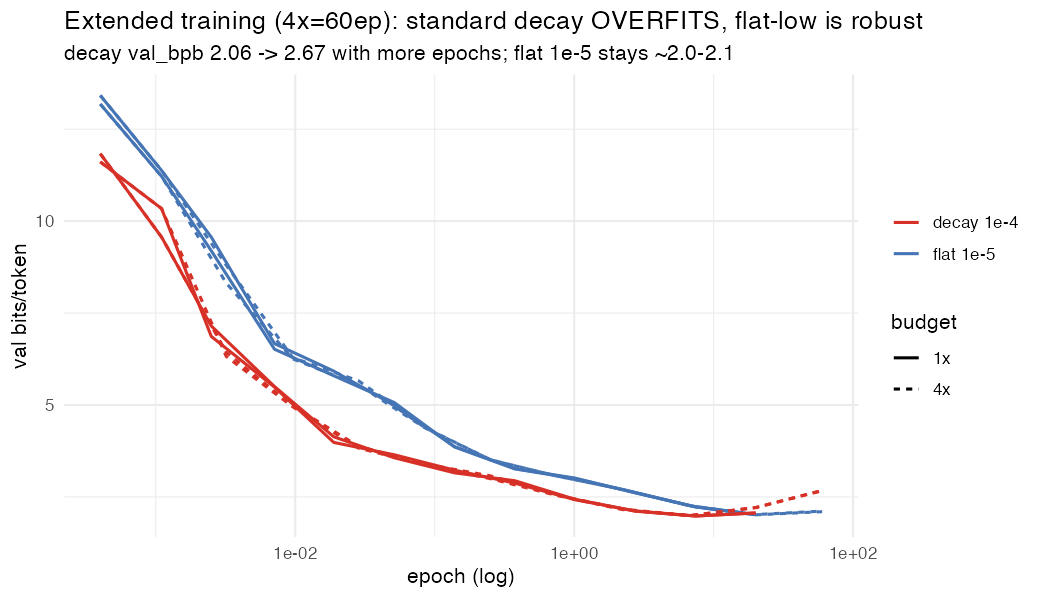
\includegraphics[width=\textwidth]{fig_overfit_4x.png}\\[-0.2em]
\caption{(3) 4$\times$: decay overfits, flat-low robust.}\label{fig:overfit}
\end{minipage}\hfill
\begin{minipage}{0.49\textwidth}\centering
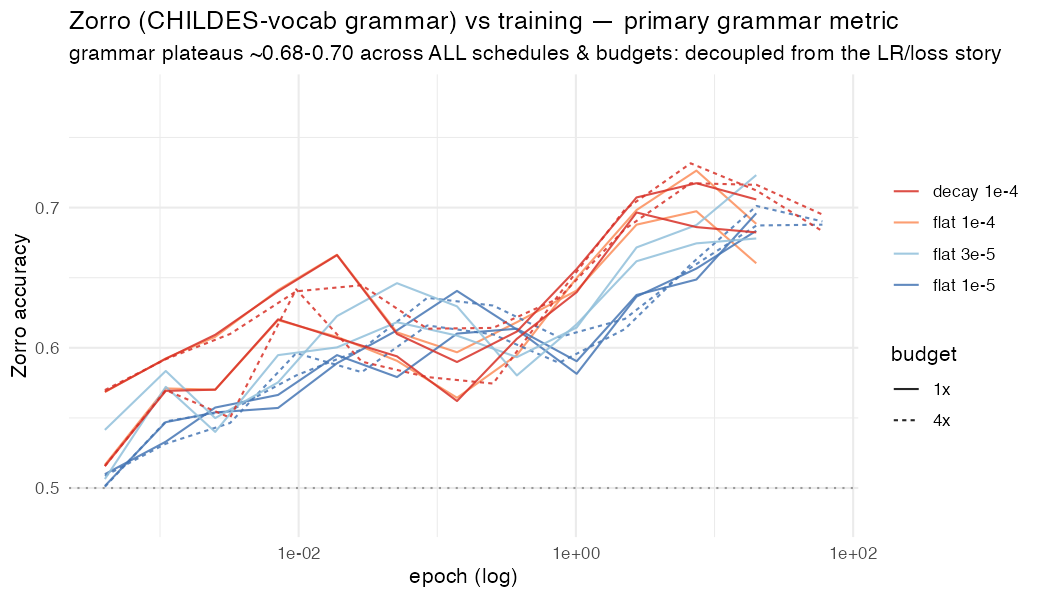
\includegraphics[width=\textwidth]{fig_zorro.png}\\[-0.2em]
\caption{(4) grammar (Zorro) decoupled.}\label{fig:zorro}
\end{minipage}
\end{figure}

\section{Interpretation}
On CHILDES the flat-low-LR ``acceleration'' is, to first order, an \textbf{optimization / regularization}
phenomenon: a gentle constant LR in the multi-epoch small-data regime \emph{de-front-loads lexical
accumulation and avoids overfitting}, which is why it simultaneously raises \J{}, lowers validation loss,
and is robust to extended training. But the decisive negative is finding (4): \textbf{none of this transfers
to grammatical competence}. Zorro is flat across every arm. So the intervention does \emph{not} make the
model a better \emph{structural} learner --- it changes \emph{when} and \emph{how cleanly} the lexical
distribution is absorbed, not what grammar is learned.

This sharpens the open question from Phase 1 in the useful direction. The kid-like reading of increasing
returns is ``learning-to-learn'': earlier structure makes later structure easier, which should manifest as
\emph{compounding capability} (grammar, generalization). What flat-low LR delivers is increasing returns on
the \emph{lexical-accumulation} axis, \textbf{decoupled} from capability. For the paper's argument this is
the clean statement: an LM \emph{can} be pushed to show the kid-like \J{} signature on word learning, but
via an optimization knob that leaves grammatical competence untouched --- evidence that the LM ``acceleration''
is mechanistically different from the child's, not just smaller.

\section{Novel-word acquisition --- a direct learning-to-learn test}
The question left open above is whether the flat-low regime makes a \emph{better learner} or merely a
less-overfit model. We tested it directly, reusing the saved checkpoints. From each of the 12 checkpoints
we warm-started and continued training under an \textbf{identical} protocol (same held-out CHILDES carrier,
same constant LR $10^{-5}$, same data order) on a corpus seeded with 24 \textbf{novel words} introduced by
nonce-substitution (e.g.\ \emph{blicket} placed in \emph{car}'s contexts) at controlled frequency. The
models have never seen these forms; we log per-nonce surprisal and take the \textbf{floor} reached after a
fixed $\sim$100 exposures (lower = better learned). The decisive control: regress mastery on the source
checkpoint's \textbf{J} (returns signature) \emph{and} its starting \textbf{val\_bpb} (competence) --- if J
predicts new-word mastery \emph{beyond} competence, that is learning-to-learn, not just a healthier model.

\textbf{Result (Fig.~\ref{fig:nonce}): new-word mastery tracks the regime, not competence.} The floor
correlates strongly with J ($r=-0.80$); in \texttt{lm(floor\,$\sim$\,J + val\_bpb)} the J coefficient is
significant ($-2.51$, $p=0.026$) while val\_bpb is not ($p=0.51$). Flat-low (high-J) checkpoints learn
genuinely new words to a lower floor than decay or flat-full, and the badly-overfit decay-4$\times$
checkpoints (high val\_bpb but $J<0$) are the \emph{worst} new-word learners \emph{despite the most
training}. So the flat-low regime leaves a model that is specifically better at \emph{acquiring new
vocabulary}, dissociable from its overall loss. (A within-run variant --- are later-introduced nonce
cohorts learned faster? --- is null once forgetting is controlled, as expected for a converged model
re-seeing known data: the effect lives \emph{across} regimes, not within one short continuation.)
Caveat: 12 checkpoints, and J/val\_bpb are correlated, so this is a strong-but-not-airtight dissociation;
the simple $r$ ($-0.80$ for J vs $+0.63$ for competence) is the most robust summary.

\begin{figure}[h]\centering
\begin{minipage}{0.49\textwidth}\centering
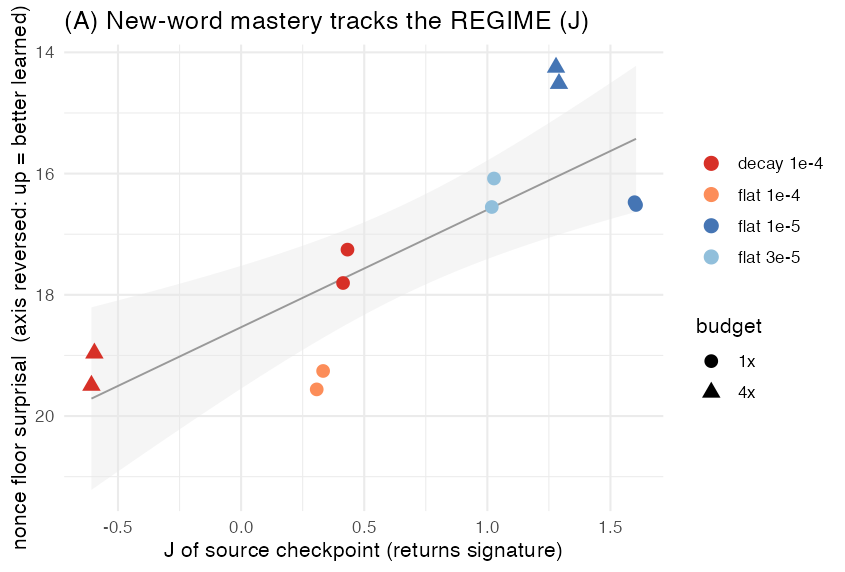
\includegraphics[width=\textwidth]{fig_nonce_regime_J.png}\\[-0.2em]
\caption{new-word mastery vs regime (J).}\label{fig:nonce}
\end{minipage}\hfill
\begin{minipage}{0.49\textwidth}\centering
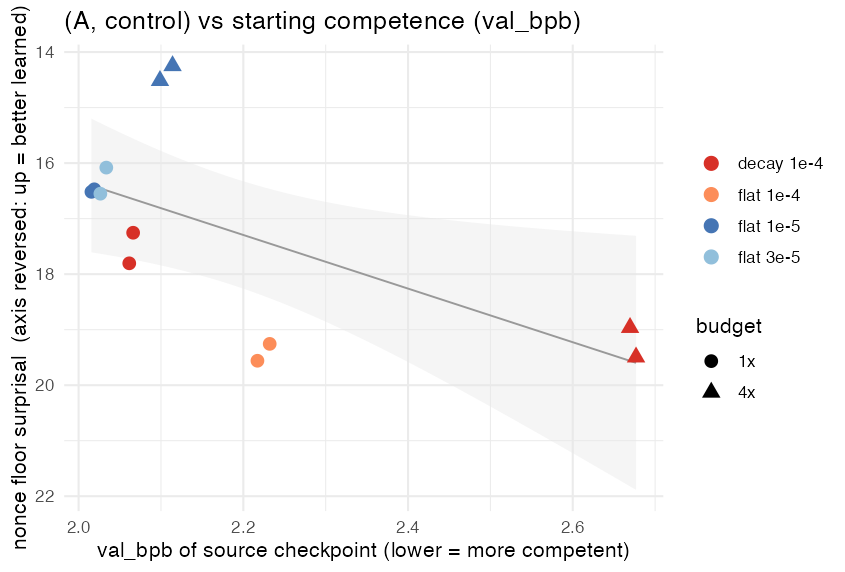
\includegraphics[width=\textwidth]{fig_nonce_regime_valbpb.png}\\[-0.2em]
\caption{control: vs starting competence (weaker).}\label{fig:noncectl}
\end{minipage}
\end{figure}

\textbf{Refined verdict.} Combining everything: the flat-low schedule \textbf{enhances the lexical-learning
faculty specifically} --- it yields the kid-like increasing-returns J on known words \emph{and} makes the
model a faster learner of genuinely new words (tracking the regime, not competence) --- while leaving
\textbf{grammatical competence untouched} (Zorro flat across all arms). ``Lexical learning-to-learn,
syntactically inert.'' That is a sharper and more interesting claim than either ``it's just optimization''
or ``the LM accelerates like a child.''

\section{What this buys the paper / next steps}
\begin{itemize}[nosep,leftmargin=1.2em]
\item A concrete, reproducible demonstration that the flat-low regime produces a genuinely better
\emph{word}-learner (lexical \J{} \emph{and} faster new-word acquisition, tracking regime not competence)
but moves grammar not at all --- a precise statement of how the LM ``acceleration'' is and isn't kid-like.
\item The decisive learning-to-learn test is now \emph{done} ($\S6$) and positive; firm-ups: a second
nonce-corpus seed (word-level CIs), a higher continuation LR to amplify, and a genuinely-novel-concept
version (nonce words in \emph{novel} roles, not fast-mapping into known slots).
\item Worth a look: a CHILDES-vocabulary-\emph{filtered} BLiMP for a sharper broad-syntax readout; and
whether any intervention moves \emph{grammar} trajectories at all (none here did).
\end{itemize}

\section*{Reproducibility}
All code/data under \texttt{studies/llm/}: sandbox sweep + scorer in \texttt{autoresearch\_pilot/}
(\texttt{returns\_score.R}, \texttt{bank\_results.tsv}, \texttt{RESULTS.md}); CHILDES experiment in
\texttt{childes\_flatlr/} (\texttt{train\_gpt2\_childes\_flatlr.py}, \texttt{eval\_grammar.py},
\texttt{grammar\_callback.py}, \texttt{run\_arm.sh}, \texttt{dispatch\_arms.sh}, \texttt{manifest\_\{1x,4x\}.txt},
\texttt{analyze.R}, \texttt{endpoints.csv}). Runs on ccn2 at \texttt{/data2/mcfrank/ladder/flatlr\_grammar/runs/}.
12 arms, 0 failures; Zorro = 23 CHILDES-vocab paradigms, BLiMP = 67 paradigms (minimal-pair log-prob scoring).
\end{document}
